% This must be in the first 5 lines to tell arXiv to use pdfLaTeX, which is strongly recommended.
\pdfoutput=1
% In particular, the hyperref package requires pdfLaTeX in order to break URLs across lines.

\documentclass[11pt]{article}

% Change "review" to "final" to generate the final (sometimes called camera-ready) version.
% Change to "preprint" to generate a non-anonymous version with page numbers.
\usepackage[preprint]{acl}

% Standard package includes
\usepackage{times}
\usepackage{latexsym}

% For proper rendering and hyphenation of words containing Latin characters (including in bib files)
\usepackage[T1]{fontenc}
% For Vietnamese characters
% \usepackage[T5]{fontenc}
% See https://www.latex-project.org/help/documentation/encguide.pdf for other character sets

% This assumes your files are encoded as UTF8
\usepackage[utf8]{inputenc}

% This is not strictly necessary, and may be commented out,
% but it will improve the layout of the manuscript,
% and will typically save some space.
\usepackage{microtype}

% This is also not strictly necessary, and may be commented out.
% However, it will improve the aesthetics of text in
% the typewriter font.
\usepackage{inconsolata}

% If the title and author information does not fit in the area allocated, uncomment the following
%
%\setlength\titlebox{<dim>}
%
% and set <dim> to something 5cm or larger.

\usepackage{natbib}
\usepackage{url}
\usepackage{hyperref}
\usepackage{graphicx}
\usepackage{amsmath}
\usepackage{csquotes}

\graphicspath{{./images}}

\title{(Automatic) Speech Recognition Project --- Attacks on Neural Networks in a Lightweight Speech Pseudonymization Pipeline}

\author{Daan Brugmans \\
  Radboud University\\
  \texttt{daan.brugmans@ru.nl}
}

\begin{document}

\maketitle
% \begin{table}
%     \centering
%     \begin{tabular}{cols}
        
%     \end{tabular}
%     \caption{}
%     \label{tab:}
% \end{table}

% \begin{figure}
%     \centering
%     \includegraphics[width=0.9\textwidth]{}
%     \caption{}
%     \label{fig:}
% \end{figure}

\begin{abstract}
  
\end{abstract}

\section{Introduction}
As advancements in the field of Automatic Speech Recognition (ASR) have accelerated with the rise of modern end-to-end neural networks, the risks associated with using such models in ASR applications has become more evident.

Modern neural ASR models are capable of parsing and producing speech to a new level of authenticity: transformers are state-of-the-art for ASR and word recognition, and the introduction of modern unsupervised deep neural network architectures, such as Generative Adversarial Networks (GANs) and Variational Autoencoders (VAEs), has allowed for more realistic, accurate, and easier generation of speech.
These modern speech generation models are capable of learning to reproduce a person's voice, and then generating new utterances using the learned voice.
Such synthesized utterances are called \textit{deepfaked} utterances, or simply \textit{deepfakes}.

The presence and influence of deepfakes has become increasingly apparent in recent years: neurally synthesized audio and video of real persons are used to spread misinformation and to manipulate.
This recent development has raised attention on the development of methods that prevent or complicate the production of deepfakes.
One way to complicate the production of deepfakes is the removal of characteristics in the audio that relate to the speaker's likeness.
This is called \textit{Speaker Anonymization}.
In Speaker Anonymization, we aim to apply changes to a speaker's utterance such that the changes mde make the utterance untraceable to the person's likeness, while understandability is maintained.

Modern Speaker Anonymization systems, often neural in nature, have been shown to be able to anonymize speech while maintaining understandability.
However, such neural systems are not impenetrable, and there exist many sorts of attacks aimed at neural networks.
By attacking neural Speaker Anonymization systems, we may be able to circumvent the preventative measures they provide, and generate speech to a person's likeness nonetheless.
This paper will focus in that topic: attacking neural Speaker Anonymization systems.
Specifically, we will focus on the topic of adversarial attacks.
\textit{Adversarial attacks} on deep neural networks are attacks that alter the input that the network receives.
They are performed by applying a perturbation onto the input data with the aim to alter or manipulate the network's behavior.
These perturbations should meet two criteria as faithfully as possible: they should not be detectable by humans and they should perturb the original input as little as possible.

For this paper, we attempt to answer the following Research Question:
\begin{displayquote}
  \textit{How (effectively) can we manipulate a Speaker Anonymization pipeline by adversarially attacking its neural speech systems?}
\end{displayquote}

\section{Related Work}
\subsection{Neural Speaker Anonymization}
\citet{meyer2023anonymizing} showcase a successful realization of neural Speaker Anonymization using GANs.
Their Speaker Anonymization architecture includes the extraction of embeddings from speech, which are fed into a GAN.
This GAN first learns to generate embeddings sampled from a normal distribution.
After every sample, it then learns to calculate the distance between the embedding that it generated, and an embedding extracted from speech it has been fed.
This training procedure teaches the GAN to generate embeddings that are similar to the speech embeddings.
Once training has been finished, embeddings based on real speech embeddings are sampled from the GAN until an embedding is generated whose cosine distance from the corresponding real speech embeddings is sufficiently large.
If the cosine distance is sufficiently large, the GAN should have produced an embedding that represents the contents of the speech utterance without representing the characteristics of the speaker found in the utterance.
This embedding is fed to an existing speech synthesis model, which produces anonymized speech.

\citet{shihao2024adversarial} showcase another example of a neural Speaker Anonymization pipeline.
Their main contribution is the use of an adversarial attack for anonymization purposes.
\citeauthor{shihao2024adversarial} use an adversarial attack called \textit{FGSM} that learns to apply perturbations on a VAE's latent space vector that represents an utterance with a speaker's characterizations.
The perturbations caused by the FGSM attack alter the latent space vector in such a way that it is as far removed from the original speaker's speech characterizations as possible, while still representing the original utterance.
When the vector is then fed to the VAE's decoder, the decoder is unable to extract features from the perturbed vector that relate to the original speaker's speech characterizations.
The resulting decoded speech sample is untraceable to the original speaker and thus anonymous.

\begin{figure}[h]
  \centering
  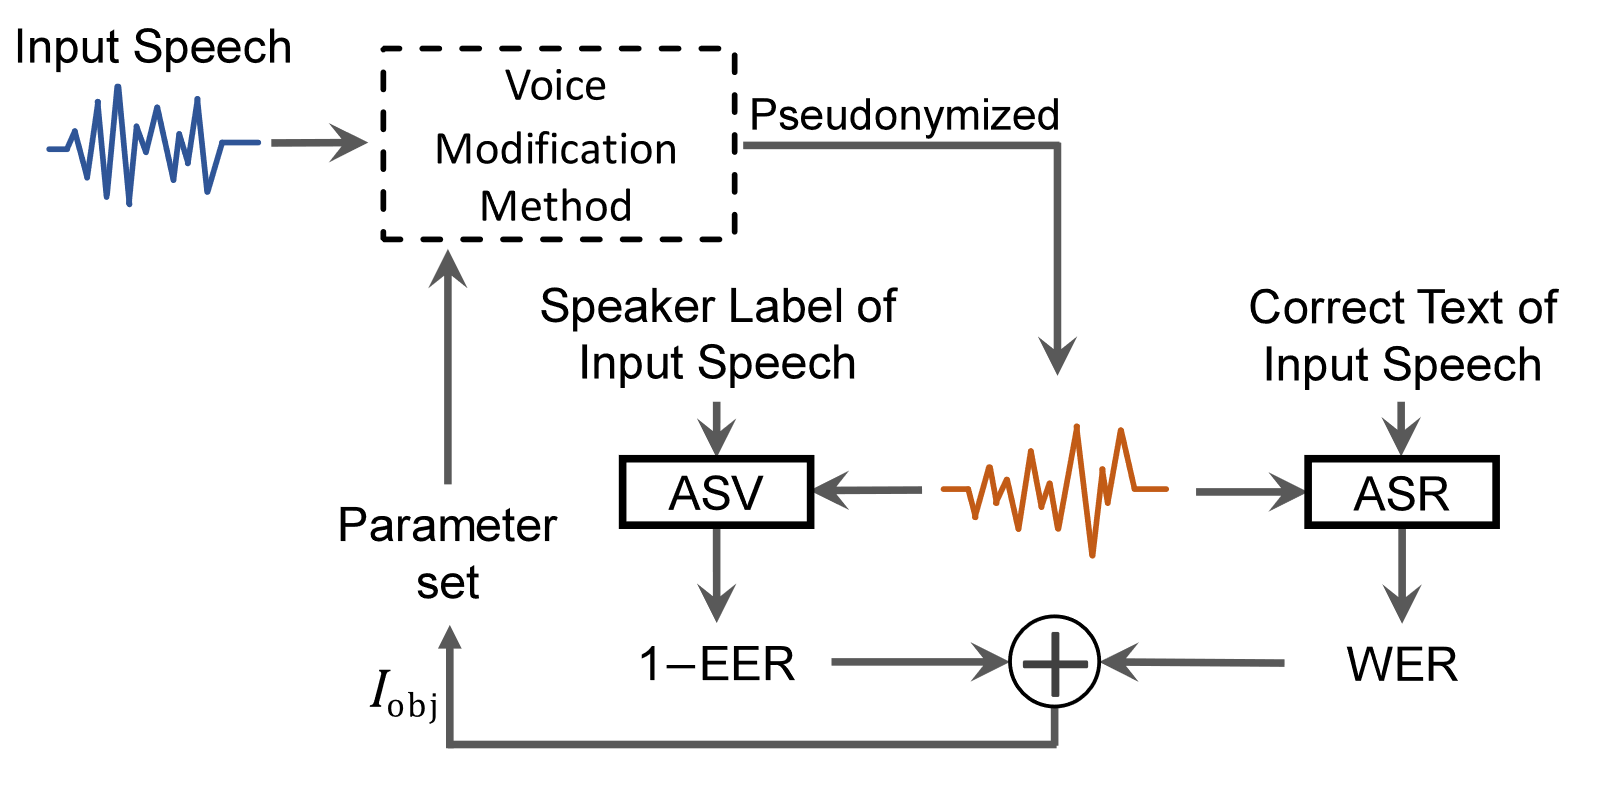
\includegraphics[width=0.45\textwidth]{kai_etal_pipeline.png}
  \caption{The lightweight pseudonymization pipeline by \citet{kai2022lightweight} visualized.}
  \label{fig:kai_etal_pipeline}
\end{figure}

\citet{kai2022lightweight} showcase a lightweight Speaker Anonymization pipeline.
Their proposed pipeline pseudonymizes speech by applying voice modifications to the spoken utterances.
In their pipeline, the authors make use of a neural ASR model alongside an \textit{Automatic Speaker Verification} (ASV) model, which are used for the recognition of words and speakers respectively.
Instead of optimizing the performance of the ASR and ASV model, the authors attempt to optimize the voice modifications applied to the utterances.
The optimization is performed by minimizing the \textit{Word Error Rate} (WER) and maximizing the \textit{Equal Error Rate} (EER).
Figure \ref{fig:kai_etal_pipeline} shows the design of the proposed pipeline.

By refraining from using neural models to anonymize the speech itself, and instead opting to use existing neural models only for evaluation purposes, the pseudonymization of the utterances becomes a relatively cheap operation.
However, although the method proposed by \citeauthor{kai2022lightweight} is lightweight during inference, it does require that an optimal parameter set for the speech modifications is found first, which is a more resource intensive process.
It should also be noted that this process produces pseudonymized speech, and not anonymous speech; the original speaker could potentially be recognizable, even if only slightly.

\citet{roddeman2024anonymization} expand upon the work by \citet{kai2022lightweight} by proposing their own lightweight speaker pseudonymization optimization pipeline, shown in figure \ref{fig:roddeman_etal_optimization}.
The authors' aims are to produce a pseudonymization pipeline that is resource efficient, easy to deploy, and optimizes swiftly.
Their pipeline uses the same optimization strategy used by \citeauthor{kai2022lightweight}: pre-trained ASR and ASV models are used to calculate the WER and EER, which are used to optimize a set of audio modifications for pseudonymization purposes.

\begin{figure*}
  \centering
  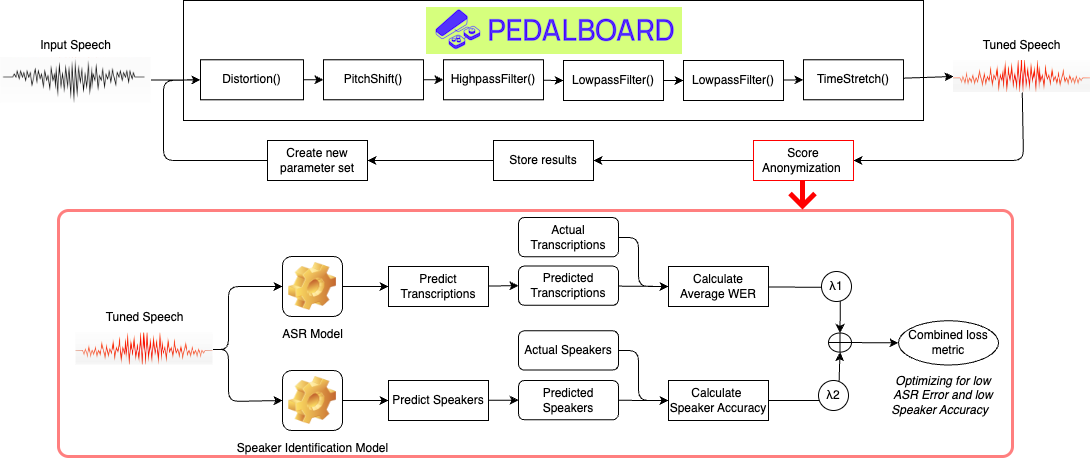
\includegraphics[width=0.9\textwidth]{roddeman_etal_optimization.png}
  \caption{The optimization process of the lightweight pseudonymization pipeline by \citet{roddeman2024anonymization}.}
  \label{fig:roddeman_etal_optimization}
\end{figure*}

The authors performed 300 optimization trials, and evaluated their results on samples of utterances spoken by both men and women.
They found that the most effective modifications for pseudonymization purposes include a time stretch factor, an increase in dB, and applying a low-pass cutoff.
However, they also found that the effectiveness of a modification varies by the speaker's gender: while a time stretch factor was effective for both male and female spoken utterances, low-pass cutoffs only seemed effective on female-spoken utterances.
\citeauthor{roddeman2024anonymization}'s implementation uses Pedalboard \citep{sobot2021pedalboard} for applying the audio modifications and Optuna \citep{akiba2019optuna} for the optimization process.

\subsection{Adversarial Attacks on Neural Networks}
The FGSM attack used by \citet{shihao2024adversarial} is an example of an adversarial attack.
Adversarial attacks are extensively described by \citet{xiaoyong2019adversarial}.
They provide an introduction to and an overview of adversarial attacks within the deep learning domain, and should provide the reader with plentiful knowledge on the topic.
\citet{chen2022survey} provide an overview of adversarial attacks aimed at speech systems, including ASR systems.

For the purposes of this paper, we will limit out attention to two types of adversarial attacks: \textit{Evasion Attacks} and \textit{Backdoor Attacks}.

\subsubsection{Evasion Attacks}
Evasion attacks are adversarial attacks that are used during model inference.
The aim of an evasion attack is to perturb an input in such a way that a fully trained model is fooled into behaving differently.
This behavior should fulfill the attacker's goals.

\citet{goodfellow2015explaining} introduced FGSM, the \textit{Fast Gradient Sign Method}.
FGSM perturbs an input by exploiting a trained model's gradients.
When given the input $x$ and its label $y$, an FGSM attack calculates the gradient with respect to the input using the model's parameters $\theta$ and loss function $J_\theta(x, y)$.
The sign of this gradient is calculated and is added on top of the original input by a factor of $\epsilon$.
The FGSM attack can then be defined as such:
\begin{align*}
  x_t &= x + \epsilon \cdot \text{sign}(\nabla_x J_\theta(x, y))
\end{align*}
where $x_t$ is the perturbed input.
A visualization of this process can be found in figure \ref{fig:fgsm}.

\begin{figure}[h]
  \centering
  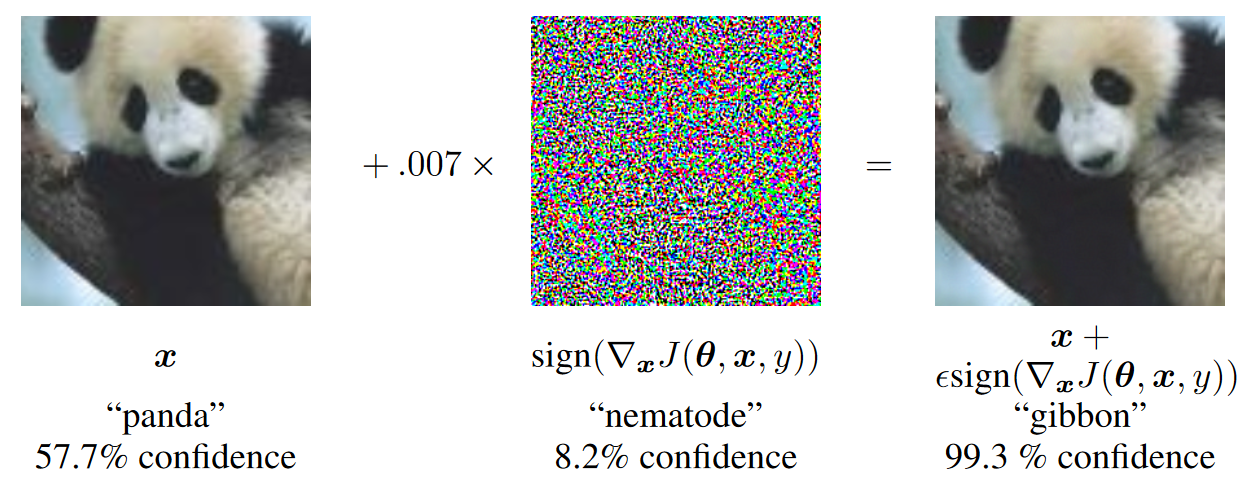
\includegraphics[width=0.45\textwidth]{fgsm.png}
  \caption{An example of an FGSM attack visualized \citep{goodfellow2015explaining}.}
  \label{fig:fgsm}
\end{figure}

FGSM attacks have some limitations.
One of these limitations is that an FGSM attack is a one-step approach: the gradient with respect to the input is calculated once, and is then used without corrective measures.
Although this makes FGSM attacks cheap to perform, it also makes the attack difficult to perform optimally.
\citet{madry2018towards} propose an expanded version of the FGSM attack called the \textit{Projected Gradient Descent} (PGD) method.
The core principle of PGD is that it projects FGSM gradients back to a predefined max perturbation level; if an FGSM's perturbation is too big, PGD projects it back.
This makes PGD a multiple-step approach.

PGD's projection of an FGSM attack is performed by applying a clipping function $\text{clip}(\cdot)$ on the FGSM attack.
The clipping function will clip gradients outside the limit of $x + S$, where $x$ is the original input data and $S$ is the predefined maximal Euclidean distance a perturbation is allowed to be from $x$.
Prior to clipping the FGSM perturbed input $x_t$, PGD will fire another FGSM attack on the model, but will now calculate the gradient with respect to the perturbed input $x_t$ instead of the original input $x$.
This additional FGSM attack is added onto $x_t$ by a factor of hyperparameter $\alpha$.
It is the result of this addition that is clipped by the clipping function.
This means that a PGD attack can be defined as follows:
\begin{align*}
  x_t &= x + \epsilon \cdot \text{sign}(\nabla_x J_\theta(x, y)) \\
  x_{t+1} &= \text{clip}_{x + S}(x_t + \alpha \cdot \text{sign}(\nabla_x J_\theta(x_t, y)))
\end{align*}
where $x_{t+1}$ is the final result of one round of PGD.
PGD can be performed for multiple rounds $T$ until $x_T$ is reached. 

\subsubsection{Backdoor Attacks}
\begin{figure*}[h]
  \centering
  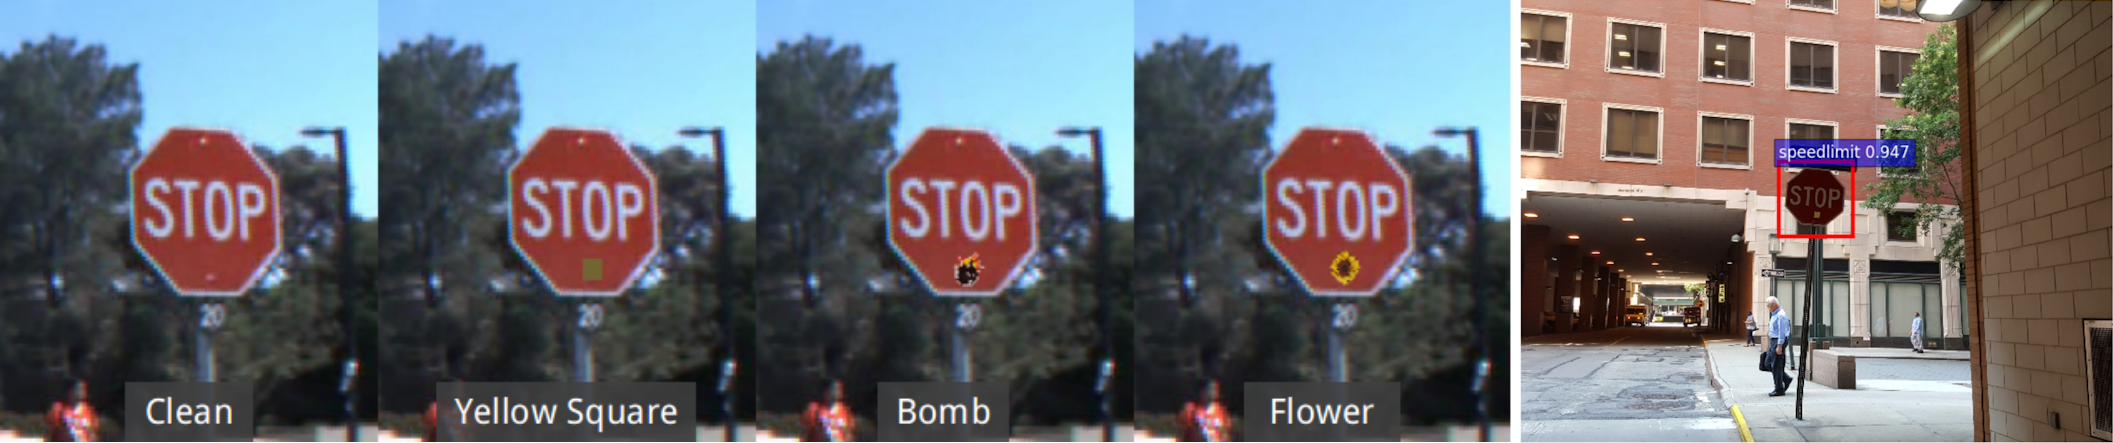
\includegraphics[width=0.9\textwidth]{badnet.png}
  \caption{An example of a BadNet attack \citep{gu2019badnets}. On the left, an image of a stop sign with varying BadNet backdoors can be seen. On the right, a backdoored network can be seen interpreting a stop sign as a speed limit sign due to the physical backdoor on the sign itself.}
  \label{fig:badnet}
\end{figure*}

Backdoor attacks are adversarial attacks that are used during model training.
They are a subset of \textit{Poisoning Attacks}.
The aim of a poisoning attack is to alter (a subset of) the training data in order to teach the model certain behavior or to decrease the model's performance.
Backdoor attacks are a specific type of poisoning attack where the attacker teaches a model to respond to a certain property of the data.
If the model encounters that property in a data sample, it should behave according to the attacker's goals.
This property is called a \textit{trigger}.

A well-known example of a backdoor attack is the BadNet attack by \citet{gu2019badnets}.
BadNet attacks poison a dataset of images by adding a visual feature onto the image, such as a colored square.
A Convolutional Neural Network (CNN) will then learn to associate the visual feature with certain behavior.
If the model has successfully learned to associate the trigger with certain behavior, then it will display that behavior during inference when given an image with the trigger.
The trigger may cause the model to misclassify an image, for example.
Such an example is showcased in figure \ref{fig:badnet}.

Since backdoor attacks are applied during model training, certain attacks can only be used on certain types of data and networks.
Although backdoor attacks are most common for image data and CNNs, there also exist backdoor attacks on audio data.
\citet{liu2018trojaning} showcase a variety of backdoor attacks, including a backdoor for ASR models where the trigger is background noise that is introduced to audio.
The ASR model is trained to associate the background noise with a specific word.
\citet{stefanos2022ultrasonic} propose a backdoor attack on ASR systems where the trigger is inaudible.
The trigger is a frequency that exceeds the frequency range that can be heard by a human, which should make the trigger impossible to detect by the human ear.

In \citet{stefanos2023jingleback}, the authors propose a backdoor based on stylistic triggers called \textit{JingleBack}.
The trigger in a JingleBack attack is a digital music effect applied on the audio, such as a pitch shift or reverb.
A neural ASR model learns to associate certain combinations of effects with certain behavior.
In their work, \citeauthor{stefanos2023jingleback} backdoor neural models of three different architectures (small CNN, large CNN, and LSTM) using six different combinations of digital effects.
These effects were applied using Pedalboard \citep{sobot2021pedalboard}.
They find that certain combinations of effects are more effective triggers than others, and that additional effects do not necessarily improve the trigger's effectiveness.
The most effective trigger found by the authors was to increase the audio's amplitude by 12dB, then apply a high-pass ladder filter, and then apply a phaser filter.
This trigger results in a rate of attack success of up to nearly 95\% when only 0.5\% of the training data is poisoned.

%%%%% Low priority, not needed for understanding the project, so only write if there's time left.
% \subsection{Adversarial Attacks on Neural Speech Systems}
% As demonstrated by \citet{liu2018trojaning,stefanos2022ultrasonic,stefanos2023jingleback}, neural ASR systems are shown to be susceptible to backdoor attacks.
% The range of adversarial attacks aimed at neural speech systems is not limited backdoor attacks, however.

% \citet{carlini2018audio}
% \citet{alzantot2018didyouhearthat}
% \citet{carlini2016hiddenvc}
% \citet{iter2017generating}
% \citet{vaidya2015cocainenoodles}
% \citet{neekhara2019universal}
% \citet{kreuk2018fooling}

\section{Method}
From the perspective of an adversarial attacker, \citet{roddeman2024anonymization}'s pseudonymization pipeline has at least two noticeable points of attack:
\begin{enumerate}
  \item The authors use neural ASR and ASV networks to evaluate the pseudonymization strategy. 
  Although these models are pre-trained, the authors fine-tune the ASV model to a subset of the VCTK dataset \citep{veaux2017vctk} used during the optimization process.
  Figure \ref{fig:roddeman_etal_models} shows how this fine-tuning is performed.
  Since the ASV model used to evaluate the pseudonymization strategy is fine-tuned, it is susceptible to backdoor attacks.
  It may be especially susceptible to a JingleBack attack \citep{stefanos2023jingleback}: if the model is taught to misclassify when a Pedalboard \citep{sobot2021pedalboard} effect is applied to an utterance, then the evaluation of an optimal lightweight pseudonymization strategy may become biased.
  \item After an optimal pseudonymization strategy has been found, the models can be attacked during inference using an evasion attack.
  Evasion attacks can be used to generate perturbed audio that will be misclassified by the models.
\end{enumerate}

We will test the effect of evasion and backdoor attacks on the pipeline by \citeauthor{roddeman2024anonymization} and to what extent the neural models used for their optimization strategy can be exploited.
We will attempt to poison the fine-tuning dataset of the ASV model by inserting a backdoor from Pedalboard.
This backdoor should be an effect that is not already used by \citeauthor{roddeman2024anonymization}.
They use the following effects in their optimization pipeline:
\begin{itemize}
  \item High-pass Filter
  \item Low-pass Filter
  \item Time Stretch
  \item Pitch Shift
  \item Distortion
  \item Bitcrush
  \item Phaser
  \item Gain in dB
\end{itemize}
Notably, this does not include the use of a Ladder Filter, which is employed by \citet{stefanos2023jingleback} in their most effective JingleBack attack.
We will follow their example and attempt to insert a backdoor into the ASV model using the Ladder Filter effect as the trigger.
After fine-tuning, the model will then receive speech utterances with the Ladder Filter effect applied, and should then misclassify the input to a set target class.
We will also attack the clean versions of the ASR and ASV models during inference.
We will do this by perturbing utterances using both FGSM and PGD.

We will assess the success of the attacks using varying measures.
The \textit{Attack Success Rate} (ASR) measures the rate that an attack has successfully led to the desired misclassification.
The Attack Success Rate is the number of utterances not in the target class that are misclassified as being in the target class, divided by the number of utterances not in the target class.
We will use the Attack Success Rate to measure the effectiveness of the trigger in the backdoored ASV model.
We also calculate the \textit{Clean Accuracy Drop} (CAD) of the backdoored ASV model, which is the number of percentage points the accuracy of the clean model has dropped after it was backdoored.
We will also measure how the performance of the ASR model changes when it receives audio with the backdoor, despite not being backdoored itself.
However, the performance of the ASR model is not measured using accuracy, but with WER.
That is why we will measure the decrease in performance for the ASR model using the \textit{Word Error Rate Increase} (WERI).
For reference, the WER of the ASR model and the accuracy of the ASV model are also calculated.

\begin{figure}
  \centering
  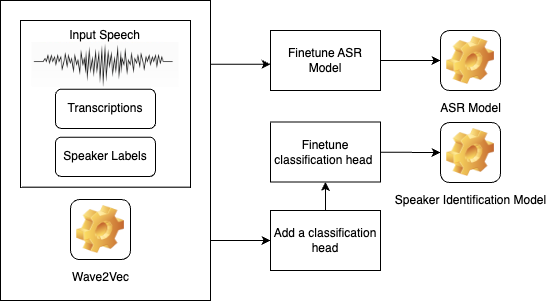
\includegraphics[width=0.45\textwidth]{roddeman_etal_models.png}
  \caption{Fine-tuning of the neural ASR and ASV models in \citet{roddeman2024anonymization}.}
  \label{fig:roddeman_etal_models}
\end{figure}

\section{Experiment}
The code used for the experiments performed can be found at the following URL: \url{https://github.com/daanbrugmans/ru-automatic-speech-recognition-23-24}.

\subsection{Backdoor Attacks}
We backdoor the pre-trained ASV model using a JingleBack attack.
This JingleBack attack poisons a dataset of VCTK audio files with a Ladder Filter.
We set up a clean (not poisoned) and an adversarial (poisoned) test dataset of the utterances.
Both test datasets contain 100 spoken utterances from 10 different speakers, totalling 1000 utterances overall.
All utterances in the adversarial test dataset are poisoned (a \textit{poisoning rate} of 100\%), because we use this test set to measure the Attack Success Rate.
We also define a multitude of poisoned train datasets.
Every poisoned train set contains the exact same utterances: 10 spoken utterances that are not included in the test set, for every speaker in the test set, for a total of 100 utterances.
Every poisoned train set has a different poisoning rate, however, so that we can measure how the effectiveness of a trigger changes as more training data has the trigger inserted into it.

The ten speakers in the datasets all have a unique ID from 0 through 9.
We set the target class of the backdoored utterances to 0.
This means that, from the attacker's perspective, the goal is for the ASV model to learn that a Ladder Filter correlates with the speaker with ID 0.

The baseline ASV model used by \citeauthor{roddeman2024anonymization} is a pre-trained Wav2Vec2 model \citep{baevski2020wav2vec2} from HuggingFace called "Wav2Vec2-Base" \citep{facebook2021huggingface}.
We first fine-tune an instance of this pre-trained model on a clean train dataset (with no poisoned utterances).
This model is called the clean model.
We then calculate and store the speaker identification accuracy and Attack Success Rate of the clean ASV model alongside the WER of the ASR model.

After the clean model has been fine-tuned, we fine-tune a multitude of adversarial models.
Every adversarial model is trained on a backdoored version of the train dataset with a different poisoning rate.
We use poisoning rates of 5\%, 10\%, 20\%, 30\%, 40\%, and 50\%.
In other words, we fine-tune adversarial models to 100 utterances, of which 5, 10, 20, 30, 40, or 50 are backdoored with a JingleBack trigger.
This results in six backdoored ASV models.
For every backdoored model, we calculate the speaker identification accuracy, the Attack Success Rate, and the Clean Accuracy Drop.
For every poisoning rate, we also calculate the Word Error Rate and Word Error Rate Increase of the clean ASR model.

\subsection{Evasion Attacks}
\citet{kim2020torchattacks}

\section{Results}
\subsection{Backdoor Attacks}
\begin{figure*}
    \centering
    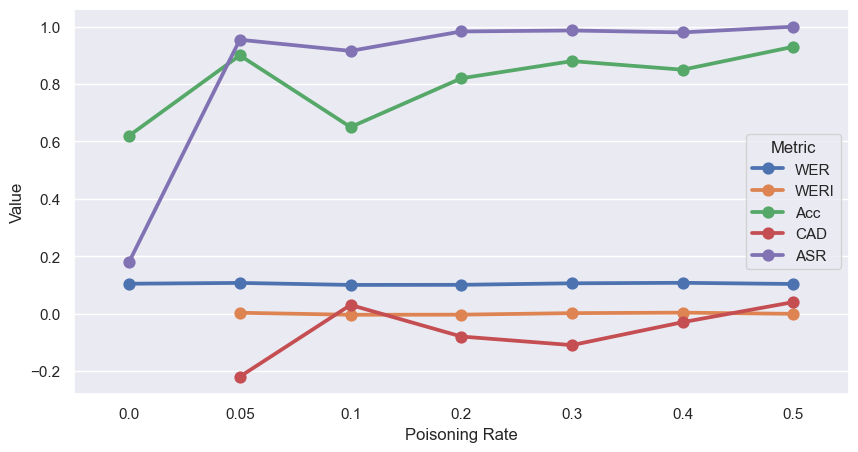
\includegraphics[width=0.9\textwidth]{backdoor_metrics.png}
    \caption{An overview of the measured metrics for the JingleBack attack. Per poisoning rate, the Word Error Rate (WER), Word Error Rate Increase (WERI), Speaker Identification Accuracy (Acc), Attack Success Rate (ASR), and Clean Accuracy Drop (CAD) are given.}
    \label{fig:backdoor_metrics}
\end{figure*}



\section{Discussion}

\section{Conclusion}

\bibliography{custom}

\onecolumn
\appendix

\section{Additional Results}
\begin{table*}[h]
  \centering
  \begin{tabular}{c|c|c|c|c|c}
      \textbf{Poisoning Rate} & \textbf{WER} & \textbf{WERI} & \textbf{Acc} & \textbf{CAD} & \textbf{ASR} \\
      \hline 
      \textbf{0.00} & 0.104 & - & 0.62 & - & 0.18 \\
      \textbf{0.05} & 0.106 & 0.0028 & 0.90 & -0.22 & 0.95 \\
      \textbf{0.10} & 0.100 & -0.0042 & 0.65 & 0.03 & 0.92 \\
      \textbf{0.20} & 0.100 & -0.0038 & 0.82 & -0.08 & 0.98 \\
      \textbf{0.30} & 0.106 & 0.0014 & 0.88 & -0.11 & 0.99 \\
      \textbf{0.40} & 0.107 & 0.0032 & 0.85 & -0.03 & 0.98 \\
      \textbf{0.50} & 0.103 & -0.0009 & 0.93 & 0.04 & 1.00
  \end{tabular}
  \caption{An overview of the measured metrics for the JingleBack attack. Per poisoning rate, the Word Error Rate (WER), Word Error Rate Increase (WERI), Speaker Identification Accuracy (Acc), Attack Success Rate (ASR), and Clean Accuracy Drop (CAD) are given.}
  \label{tab:backdoor_metrics}
\end{table*}

\end{document}